\documentclass[12pt]{book} 

\usepackage{amsmath}
\usepackage{graphicx}
\usepackage{import}
\usepackage{amsfonts}
\usepackage{booktabs}

\setlength{\parindent}{0em}  % sets auto indent at new paragraph to none

\newcommand{\incfig}[1]{%
    \import{./figures/}{#1.pdf_tex}
}

\title{\coursetitle\linebreak\lecturename}
\author{\\Cain Susko\\ 
           \\ \\ \\
      Queen's University 
    \\School of Computing\\} 

%=-=-=-=-=-title-=-=-=-=-=%
\newcommand{\lecturename}{Urban Economies And the Financialized City}
\newcommand{\coursetitle}{Urban Planning}
%=-=-=-=-=-#####-=-=-=-=-=%

\begin{document}
\begin{titlepage}
        \maketitle
\end{titlepage}


\section*{The Financialized City}
This paper will cover how economies and the industrial complex effect cities, particularly in North America. 


\section*{The Mode of Production and the History of Cities}
This section will cover the realation between economic change and the process of urbanization.
Urban development is not static and so to understand them, critical geographers analyze capitalism to 
to try and understand the changes of the city.

The structures of the current economy is based upon the economic order of cities in the past. Furthermore, the 
current iteration of economies affect the shape of urban life in cities.

\paragraph{}
The mode of production is the social and physical infrastructure for the production of goods.

Back in the middle ages, Feudalism was the mode of production in which land was the means of production. The 
social aspects of feudalism was very strict, with a strong social Heirarchy. In contrast, in the renaissance 
merchantilism was the mode of production and trade was the means.

In capitalism, the mode of production is the factory owners, and the means are the factories. The objective under
capitalism is to accumulate capital, disregarding other aspects of social and economic life.

\paragraph{}
As the industrial revolution brought on capitalism, cities grew as the means and mode of production were bought 
closer to the consumers and factories grew and some people became very wealthy, whereas others became worse off 
than before. Slums, and a general decrease in the quality of 
life for the working class emerged in this time of apparent growth and prosperous developments.


\section*{The Evolution of Cities in North America since 1800}
Cities in the United States of America can be categorized by 4 eras:
\begin{itemize}
        \item frontier-mercantile era 1700
        \item early industrial capitalism 1800
        \item national industrial capitalism 1850
        \item mature industrial capitalism 1950
        \item new economy capitalism 1970
\end{itemize}
as these eras went on, the size of cities reflected the current economic environment.

\paragraph{}
In Canada, the railroad had a large impact on inking America and Canada. Beforehand, the main link canada
had with other countries and economies was with Britain.

As this happened, there was substantial growth in the urban population with nearly 50\% of canadians living in cities
in 1850's.

As the cities and economies of canada grew, so did speculation and mercatileism. This was a golden period for 
the growth of cities (see Winnipeg in the 1800's)

This growth was at the expense of workers and their quality of life. This resulted in a strike by metal workers 
which was ended by mounties firing into the crowd and killing 3.

This should illustrate how the economies of canada has affected it's cities and how the economy can continue to 
shape the city in the future.

\section*{Urban Economies since 1945}
In the post-war era there was a ditinct change in the role of the city.
From the 50's to the 70's Fordism was prevelant in the American economy. It focused on paying workers well and 
mass production via assembly line. Additionally, policies like welfare were implemented during the post-war boom
to help increase the quality of life for (white) working class americans. The Suburd also emerged during this 
time to mirror the mas production of other goods at the time. to facilitate these new suburbs highways were
also constructed. The car replaced the person as the main concern in planning the city. As we can see the changing
post-war economy created the post-war city.
After Fordism, the knowledge based economy was introduced. This is an economy that prioritizes knowledge and information
over goods and resouces. For example: Silicon Valley. This shift was caused by a growing international economy where
wealthy countries can outsource menial tasks to lesser Coutries.
Because not everyone is a scholar--but there are no factory jobs anymore--the service sector has grown as an employer.
In an information economy, cities are incentivised to create `clusters' of industry that foster growth and development.
This economy also shifted away from the welfare state and focused policy on market oriented social support.

In Canada, the information economy maifested in the government focused on economic growth in the context of the global
economy, whereas in Forism, there was a focus on redistrubuting wealth to poorer cities to incentivise growth in them.

In the information economy, there has been a development of new living spaces: like gated communities or edge cities.
This has resulted in a large spread of population within north American cities.
\begin{figure}[h]
        \centering
        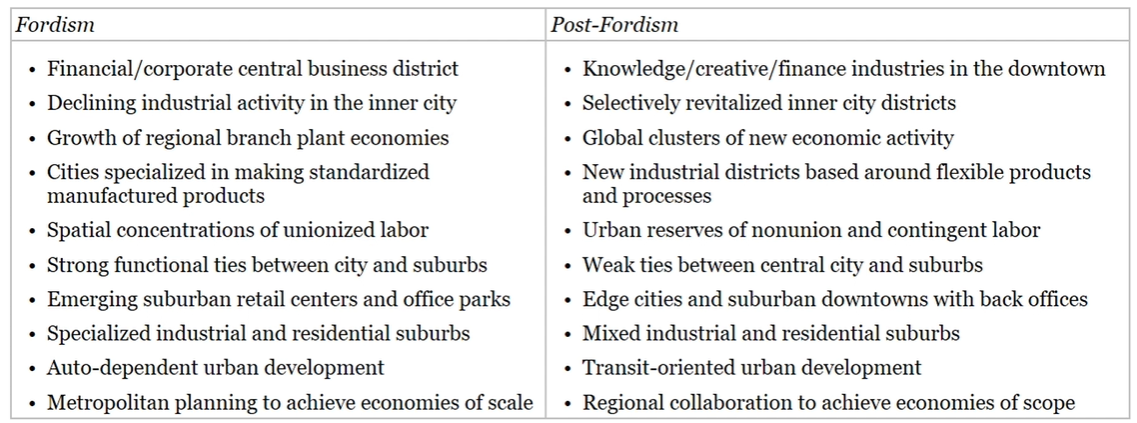
\includegraphics[scale = 0.5]{./figures/postford}
\end{figure}
\pagebreak

\section*{The Entrepreneurial City}
in the Post-Fordist era cities must compete to attract people, money and companies. This has resulted that 
cities producing the types of landscapes \textit{they} think they need, rather than the people of the city.
For example, cities would compete for Amazon to choose them to build their new Head Quarters in. New jersey
even offered to give 7 million dollars in tax breaks to if Amazon chose them.
A city has many modes of economic competition
\begin{itemize}
        \item Clustered industry
        \item Consumption/Culture
        \item Command and Control centres
        \item Governmental Redistribution
\end{itemize}

This type of competition can cause tax money to be taken away from services but can also revitalize a city (see 
the downtown of cities in north america c.2022)

The revitalization of the downtown makes a city more desirable to live in and improves the quality 
of life for it's citizens.

This spirit of competition also strengthens links in a region as many cities may work together to improve their region.
(see the Pearl River Delta cities in China).
\paragraph*{}
there are some problems with this city framework however.
The decisions made are generally outside of democracy and people have no say. Furthermore this type of governance can
lead to undesirable gentrification where not everyone in the city benefiets.

\section*{Finance and The City}
Financialization is the increasing role of financial motives, markets, actors, and institutions in a given area.
Historically, finance has had a large role in cities as well (see redlining in the US)

In the post-fordist era, cities have become more reliant on ivestment. 

In 2008 we can see this financialization as the subprime morgage which crisis caused an economic collapse.
The focus of the economy was on the buying and selling of \textit{mortgages} for homes. 
The collapse cause the housing market to tank in cities which resulted in the implosion of urban development.

\paragraph{}
in the wake of 2008, large organizations are investing in real estate in order to rent them back to the--previously--
possible owners.
Condos have also become very popular to invest and speculate on after 2008; however their vacancy is quite high
which is in contrast to the current housing crisis.
Furthermore, the finiacialization of cities can be seen as the increaing attempts of cities to decrease spending
by selling services off to private companies. (see highway 407 in Ontario)


\end{document}

